\documentclass[a4paper,11pt,UTF8]{article}
\usepackage{ctex}
\usepackage{amsmath,amsthm,amssymb,amsfonts}
\usepackage{amsmath}
\usepackage[a4paper]{geometry}
\usepackage{graphicx}
\usepackage{microtype}
\usepackage{siunitx}
\usepackage{booktabs}
\usepackage[colorlinks=false, pdfborder={0 0 0}]{hyperref}
\usepackage{cleveref}
\usepackage{esint} 
\usepackage{graphicx}
\usepackage{ragged2e}
\usepackage{pifont}
\usepackage{extarrows}
\usepackage{mathptmx}
\usepackage{float}
\usepackage{caption}
\usepackage{multirow}
\usepackage{subfigure}
\usepackage{titlesec}
\captionsetup[figure]{name={图}}
%opening
\title{数字电子技术作业(五)}
\author{谢悦晋 \quad U202210333}
\date{Nov 6th, 2023 }
\begin{document}
\maketitle
\textbf{6.2.4} 试分析图题 6.2.4 所示电路,列出状态转换表,并画出状态转换图。当输入序列$A$为01011011111111101,其输出序列 $Z$ 是什么? 该电路可以检测 $A$ 的何种输入序列?
\begin{figure}[H]
	\centering
	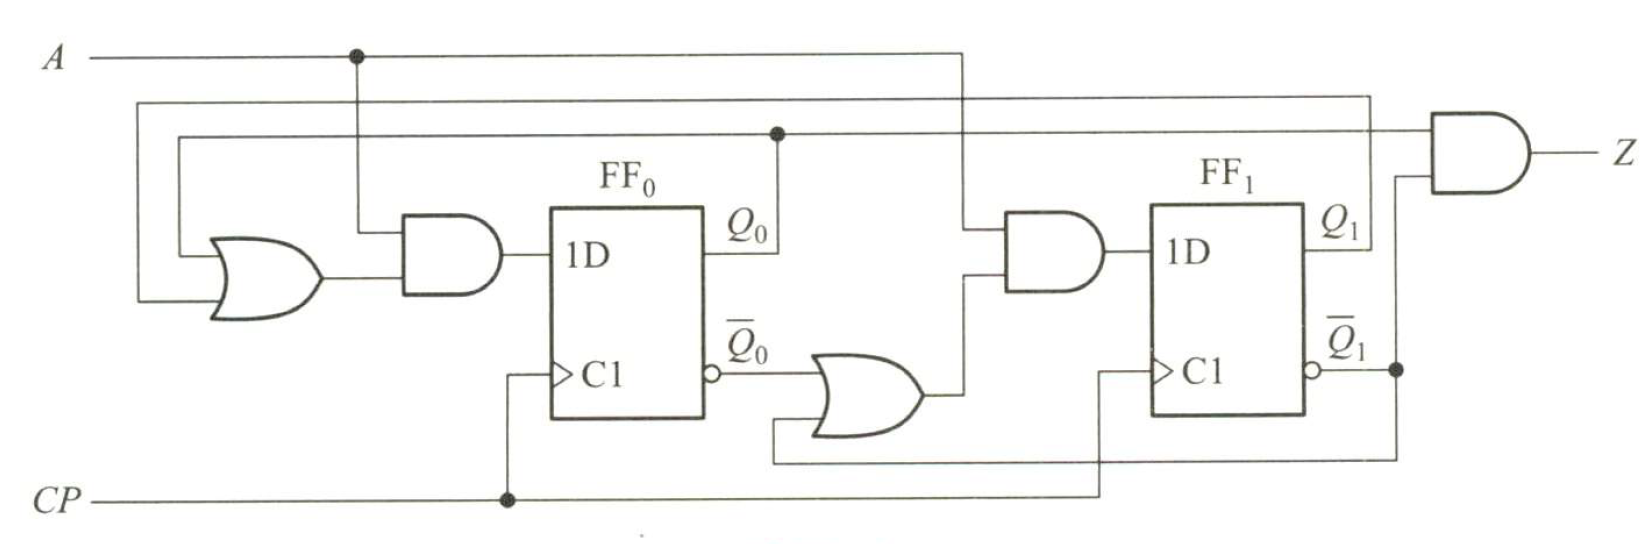
\includegraphics[width=0.9\textwidth]{6.2.4}
	\caption{6.2.4}
\end{figure}
\noindent 解:

\textbf{Step 1.} 写出输出方程,激励方程,状态方程:
$$
Z=Q_0\overline{Q}_1,
\begin{cases}
	D_{FF_0}=A(Q_1+{Q}_0)\\
	D_{FF_1}=A(\overline{Q}_0+\overline{Q}_1)
\end{cases},
\begin{cases}
	Q_{0}^{n+1}=A(Q_1^n+{Q}_0^n)\\
	Q_{1}^{n+1}=A(\overline{Q}_0^n+\overline{Q}^n_1)
\end{cases}
$$

\textbf{Step 2.} 列出状态转换表
\begin{table}[H]
	\centering
	\begin{tabular}{|c|c|c|}
		\hline
		\multirow{2}{*}{$Q_0^nQ_1^n$} & \multicolumn{2}{c|}{$Q_0^{n+1}Q_1^{n+1}/Z$}\\
		\cline{2-3}
		& A=0 & A=1\\
		\hline
		00 & 00/0 & 01/0\\
		01 & 00/0 & 11/0\\
		10 & 00/1 & 11/1\\
		11 & 00/0 & 10/0\\
		\hline
	\end{tabular}
\end{table}
\textbf{Step 3.} 画出状态转换图
\begin{figure}[H]
	\centering
	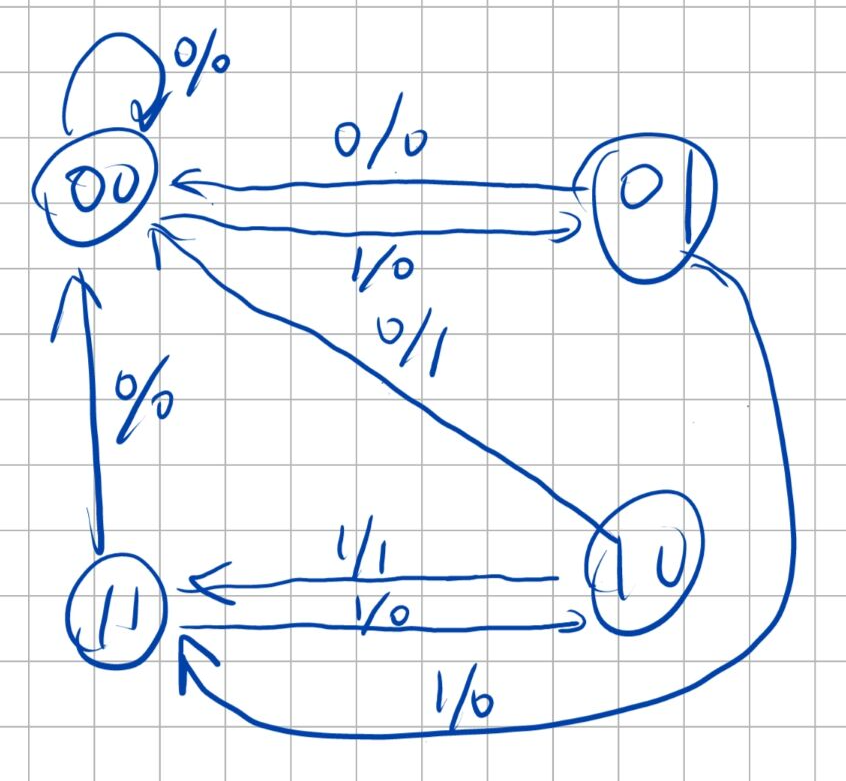
\includegraphics[width=0.5\textwidth]{6.2.4_1}
	\caption{6.2.4}
\end{figure}
输出序列为:0000 0000 0100 0101 0100,可以检测连续的三个1,若连续的三个1之后每跟着两个1就输出一个1,只要有0重新检测。

\textbf{6.2.6} 试分析图题 6.2.6 所示同步时序电路,写出激励方程组、状态转换方程组和输出方程,列出状态转换表并画出状态转换图。
\begin{figure}[H]
	\centering
	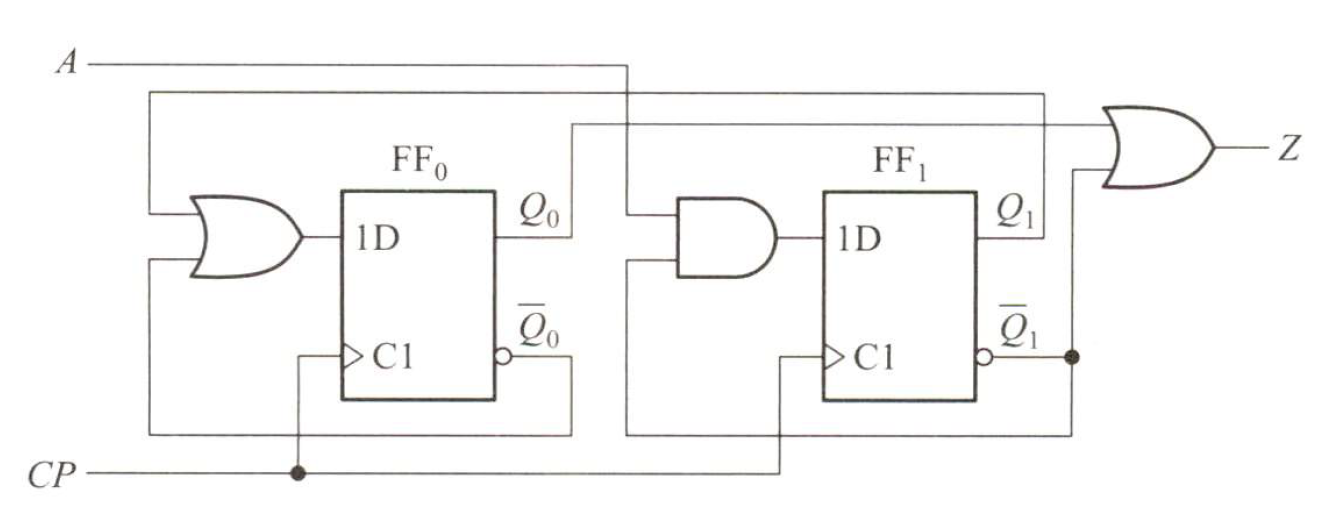
\includegraphics[width=0.9\textwidth]{6.2.6}
	\caption{6.2.6}
\end{figure}
\noindent 解:

\textbf{Step 1} 写出输出方程,激励方程,状态方程:
$$
Z=Q_0+\overline{Q}_1,
\begin{cases}
	D_{FF_0}=Q_1+\overline{Q}_0\\
	D_{FF_1}=A\overline{Q}_1
\end{cases},
\begin{cases}
	Q_{0}^{n+1}=Q_1^{n}+\overline{Q}_0^n\\
	Q_{1}^{n+1}=A\overline{Q}_1^{n}
\end{cases}
$$

\textbf{Step 2} 列出状态转换表
\begin{table}[H]
	\centering
	\begin{tabular}{|c|c|c|}
		\hline
		\multirow{2}{*}{$Q_1^nQ_0^n$} & \multicolumn{2}{c|}{$Q_1^{n+1}Q_0^{n+1}/Z$}\\
		\cline{2-3}
		& A=0 & A=1\\
		\hline
		00 & 01/1 & 11/1\\
		01 & 00/0 & 10/0\\
		10 & 01/1 & 01/1\\
		11 & 01/1 & 01/1\\
		\hline
	\end{tabular}
\end{table}
\textbf{Step 3.} 画出状态转换图
\begin{figure}[H]
	\centering
	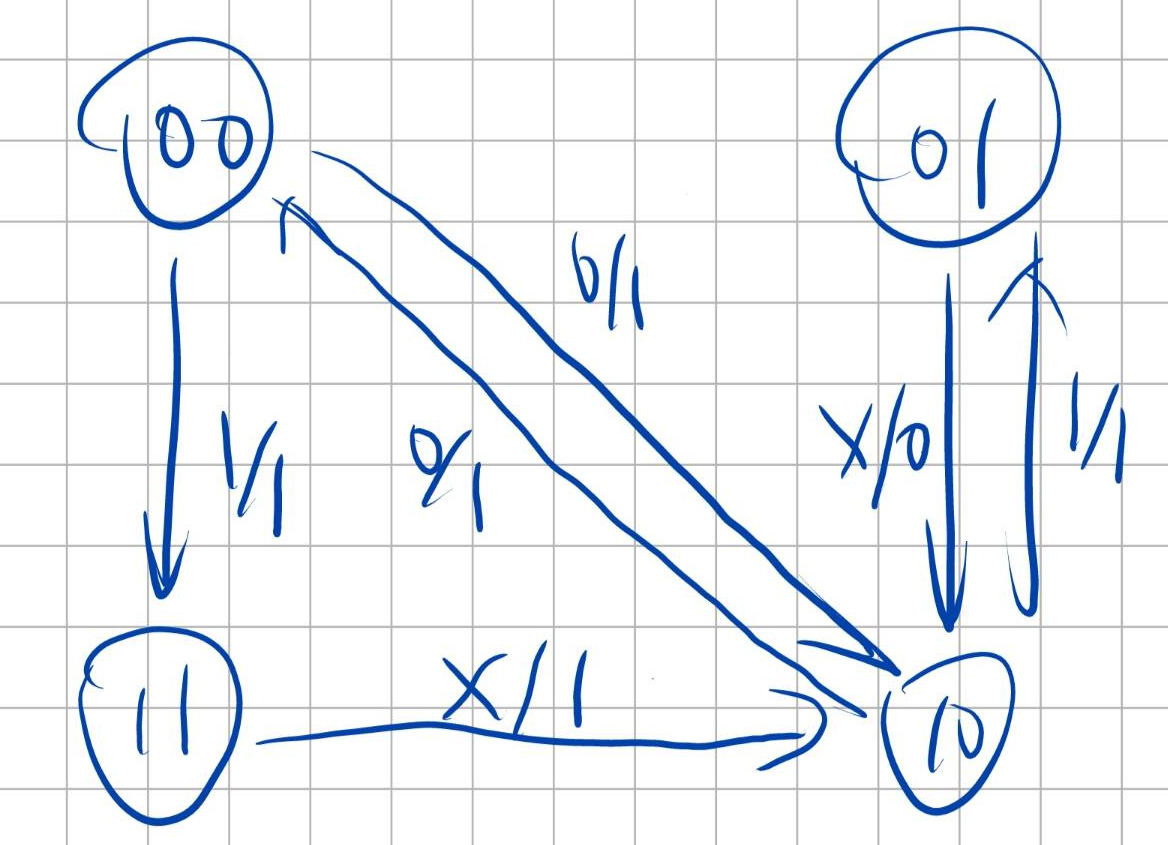
\includegraphics[width=0.5\textwidth]{6.2.6_1}
	\caption{6.2.6}
\end{figure}

\textbf{6.3.5} 试用下降沿触发的$JK$触发器和最少的门电路,实现图题 6.3.5 所示的$Z_{1}$和$Z_{2}$输出波形(要求写出Verilog程序)
\begin{figure}[H]
	\centering
	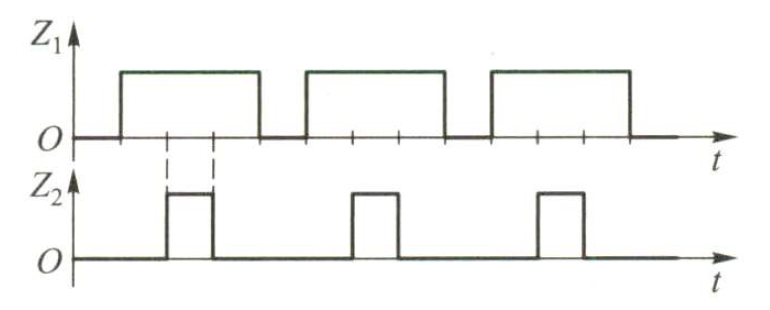
\includegraphics[width=0.7\textwidth]{6.3.5}
	\caption{6.3.5}
\end{figure}
\noindent 解:

\textbf{Step 1.} 逻辑抽象

从图6.3.5所示输出波形图可以看出,对于每一个周期,可分为4个状态:$Z_2Z_1=00,Z_2Z_1=01,Z_2Z_1=11,Z_2Z_1=01$。设定为4个状态:00,01,10,11,用两个下降沿触发的 JK 触发器实现.设两个触发器的状态为 $Q_{1}$、 $Q_0$,输出信号为$Z_1,Z_2$

\textbf{Step 2.} 列写激励方程,输出方程

首先写出真值表:
\begin{table}[H]
	\centering
	\begin{tabular}{|c|c|c|c|c|c|c|}
		\hline
		$Q_0^nQ_1^n$ & $Q_0^{n+1}Q_1^{n+1}$ & $Z_1Z_2$ & $J_0$ & $K_0$ & $J_1$ & $K_1$\\
		\hline
		00 & 01 & 00 &1&x&0&x\\
		01 & 10 & 10 &x&1&1&x\\
		10 & 11 & 11 &1&x&x&0\\
		11 & 00 & 10 &x&1&x&1\\
		\hline
	\end{tabular}
\end{table}
易得激励方程和输出方程:
$$
\begin{cases}
	J_1=K_1=Q——0\\
	J_0=K_0=1
\end{cases},
\begin{cases}
	Z_1=Q_1+Q_0\\
	Z_2=Q_1\overline{Q}_0
\end{cases}
$$

\textbf{Step 2.} 画出逻辑电路,写出Verilog语句
\begin{figure}[H]
	\centering
	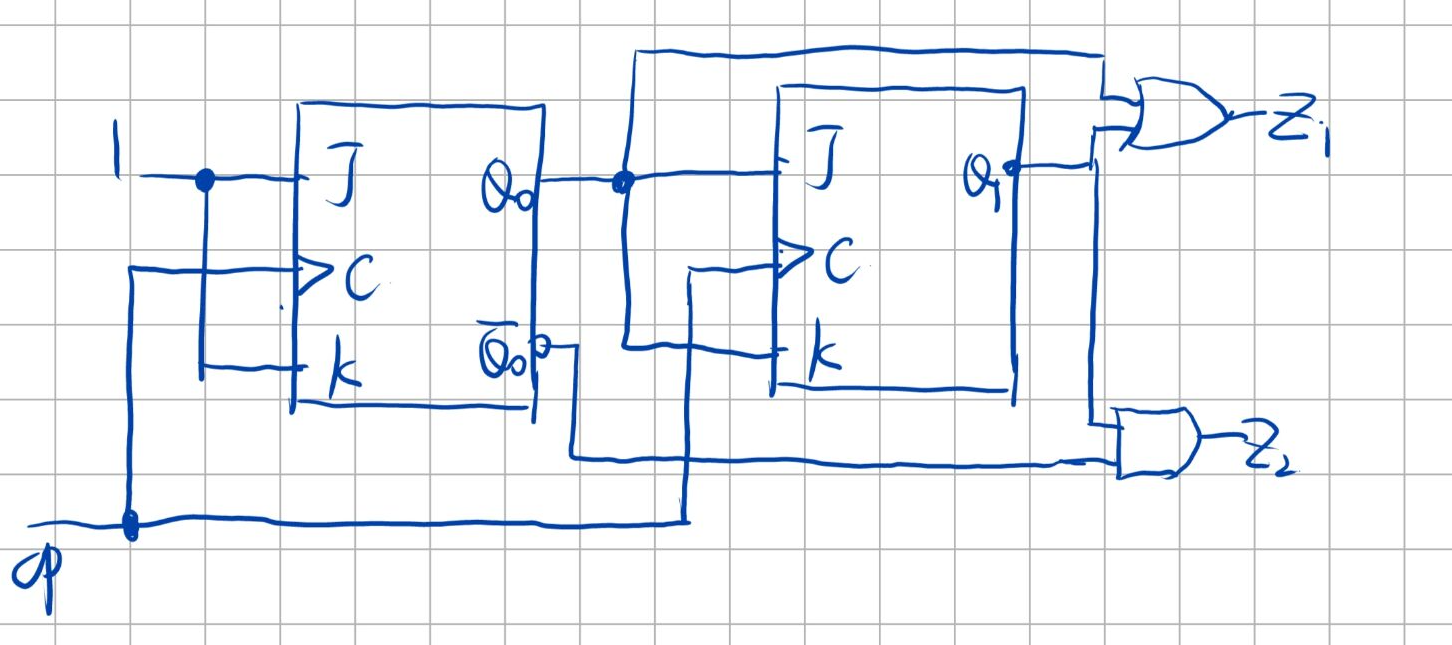
\includegraphics[width=0.7\textwidth]{6.3.5_1}
\end{figure}
\begin{figure}[H]
	\centering
	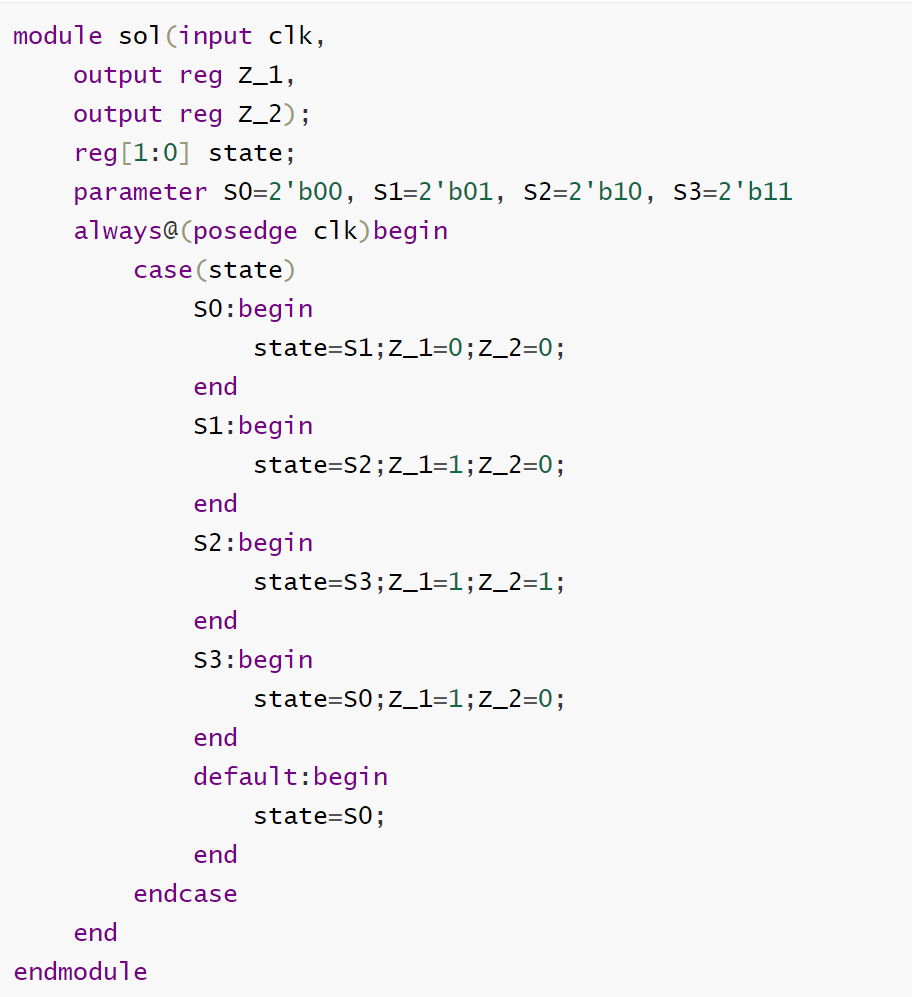
\includegraphics[width=0.7\textwidth]{6.3.5_2}
\end{figure}
\textbf{6.3.6} 试用上升沿触发的$D$触发器设计一个1101序列检测器(序列可重复),输入为串行编码序列,输出为检出信号(要求写出Verilog程序)
\noindent 解:

\textbf{Step 1.} 逻辑抽象

首先写出状态转换图和状态转换表

\begin{table}[H]
	\centering
	\begin{tabular}{|c|c|c|}
		\hline
		\multirow{2}{*}{$Q^n$} &\multicolumn{2}{c|}{$Q^{n+1}/Y$}\\
		\cline{2-3}
		& $A=0$ & $A=1$ \\
		\hline
		a&a/0&b/0\\
		b&a/0&c/0\\
		c&d/0&c/0\\
		d&a/0&e/1\\
		e&a/0&c/0\\
		\hline
	\end{tabular}
\end{table}
\textbf{Step 2.} 状态化简
\begin{table}[H]
	\centering
	\begin{tabular}{|c|c|c|}
		\hline
		\multirow{2}{*}{$Q^n$} &\multicolumn{2}{c|}{$Q^{n+1}/Y$}\\
		\cline{2-3}
		& $A=0$ & $A=1$ \\
		\hline
		a&a/0&b/0\\
		b&a/0&c/0\\
		c&d/0&c/0\\
		d&a/0&b/1\\
		\hline
	\end{tabular}
\end{table}
\textbf{Step 3.} 状态分配
\begin{figure}[H]
	\centering
	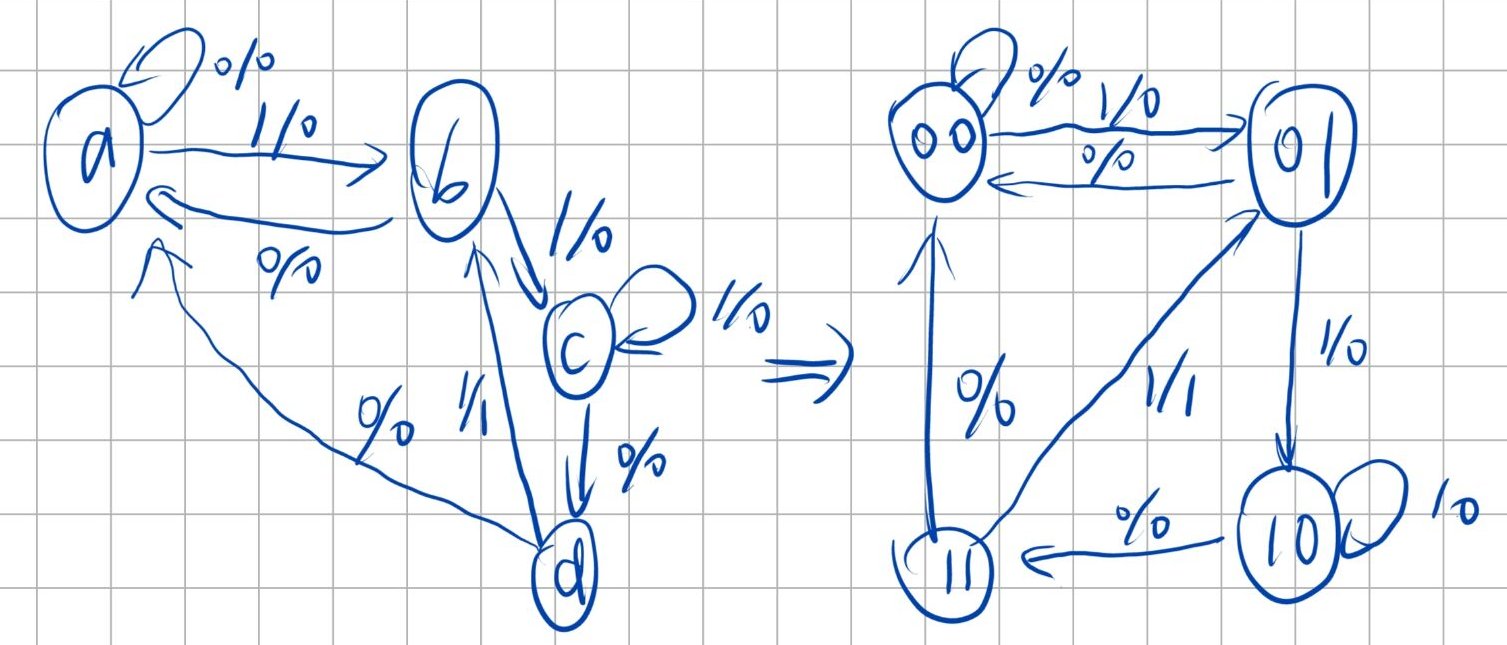
\includegraphics[width=0.8\textwidth]{6.3.6_2}
\end{figure}
\begin{table}[H]
	\centering
	\begin{tabular}{|c|c|c|}
		\hline
		\multirow{2}{*}{$Q_0^nQ_1^n$} &\multicolumn{2}{c|}{$Q_0^{n+1}Q_1^{n+1}/Y$}\\
		\cline{2-3}
		& $A=0$ & $A=1$ \\
		\hline
		00&00/0&10/0\\
		01&00/0&10/0\\
		10&11/0&10/0\\
		11&00/0&01/1\\
		\hline
	\end{tabular}
\end{table}
\textbf{Step 4.} 列写激励方程,输出方程
$$
\begin{cases}
D_{0} =A\overline{Q}_{0}Q_{1}+\overline{A}Q_{0}\overline{Q}_{1}+AQ_{0}\overline{Q}_{1} \\
D_{1} =A\overline{Q}_{0}\overline{Q}_{1}+\overline{A}Q_{0}\overline{Q}_{1}+AQ_{0}Q_{1} \\
\end{cases}
,Y=AQ_{0}^{n}Q_{1}^{n} 
$$

\textbf{Step 5.} 画出逻辑电路,写出Verilog语句
\begin{figure}[H]
	\centering
	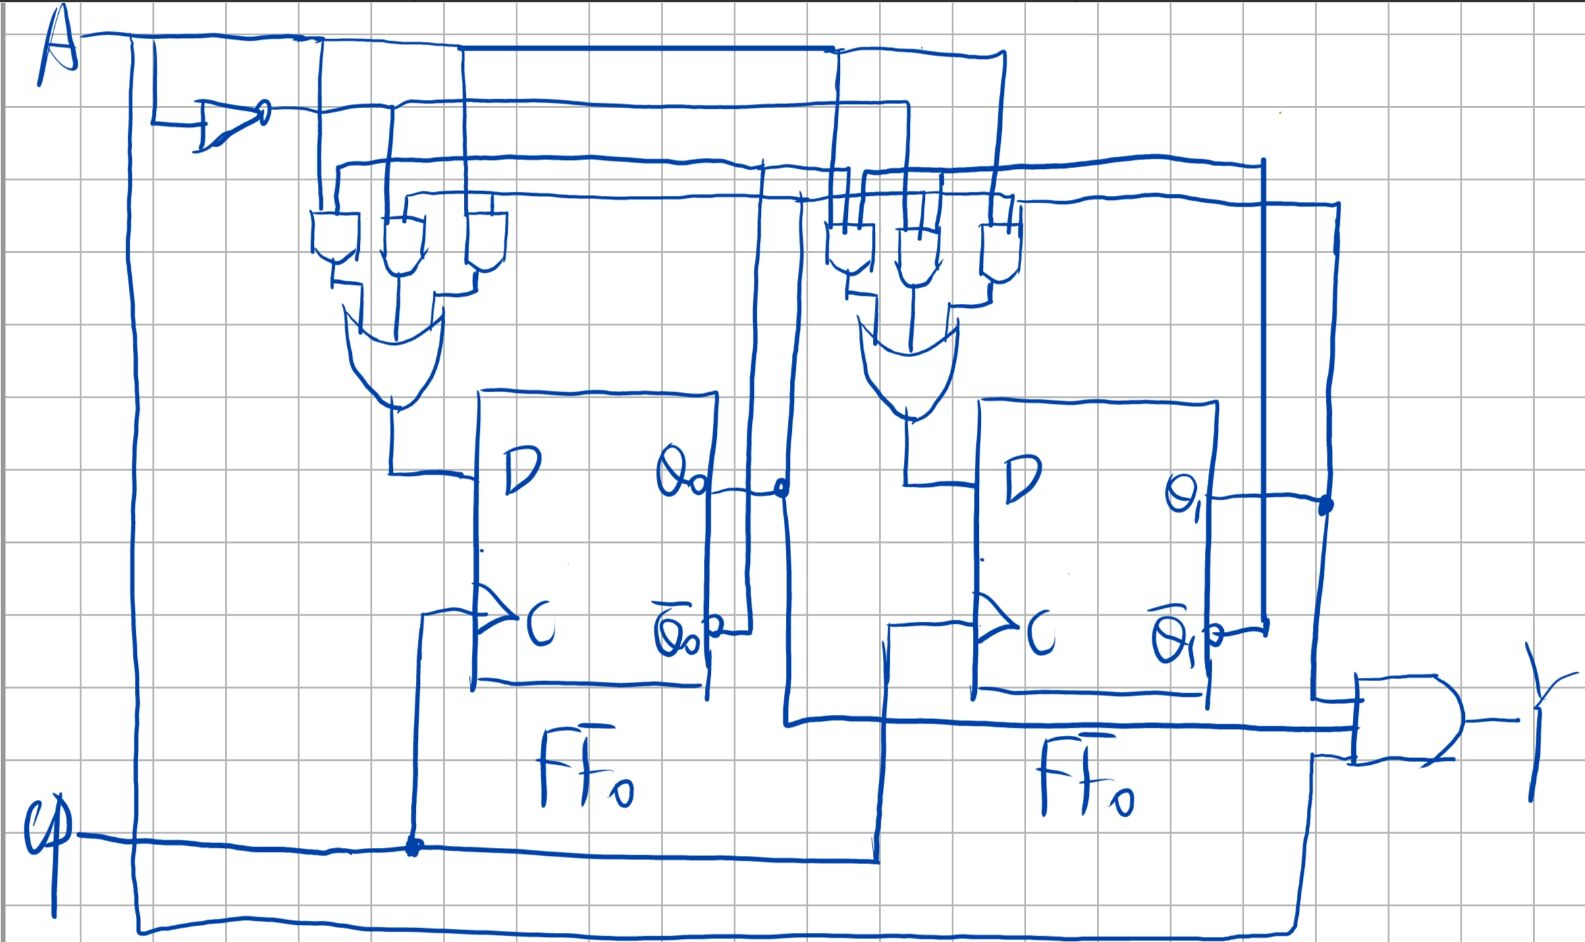
\includegraphics[width=0.7\textwidth]{6.3.6_3}
\end{figure}
\begin{figure}[H]
	\centering
	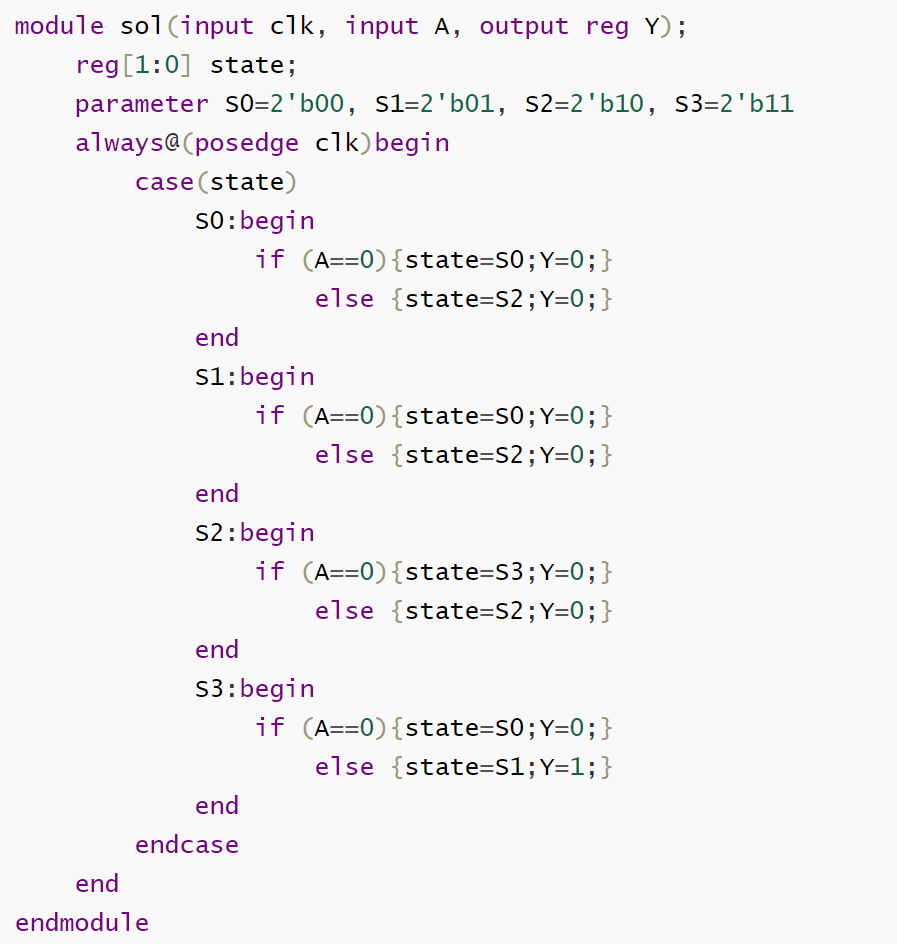
\includegraphics[width=0.68\textwidth]{6.3.6_4}
\end{figure}
\end{document}